\documentclass{ceurart}

\usepackage{acronym}
\usepackage{subcaption}

\renewcommand{\acffont}[1]{\textsl{#1}}


%%
%% end of the preamble, start of the body of the document source.
\begin{document}

%%
%% Rights management information.
%% CC-BY is default license.
\copyrightyear{2026}
\copyrightclause{Copyright for this paper by its authors.\\
  Use permitted under Creative Commons License Attribution 4.0
  International (CC BY 4.0).}

%%
%% This command is for the conference information
\conference{``Search Engines'', course at the master degree in ``Computer Engineering'', Department of Information Engineering, and at the master degree in ``Data Science'', Department of Mathematics ``Tullio Levi-Civita'', University of Padua, Italy. Academic Year 2025/2026}

%%
%% The "title" command
\title{SEUPD@CLEF: Team NEXA}

%%
%% The "author" command and its associated commands are used to define
%% the authors and their affiliations.
\author[1]{Paul Arlot}[
  email=paullouisjean.arlot@studenti.unipd.it
]

\author[1]{Andrea Di Tillo}[
  email=andrea.ditillo@studenti.unipd.it
]

\author[1]{Gaute Greiff Flagstad}[
  email=gaute.greiff.flaegstad@studenti.unipd.it
]

\author[1]{Bita Khashechian}[
  email=bita.khashechian@studenti.unipd.it
]

\author[1]{Danil Smirnov}[
  email=danil.smirnov@studenti.unipd.it
]

\author[1]{Marco Tomaiuoli}[
  email=marco.tomaiuoli@studenti.unipd.it
]

\address[1]{University of Padua, Italy}


%%
%% The abstract is a short summary of the work to be presented in the
%% article.
\begin{abstract}

  This paper presents the system developed by Team NEXA for Task 1 of the CLEF 2026 CheckThat! Lab, focusing on the retrieval of scientific sources for claims found on social media. Given the challenge of linking informal web discourse to formal scientific literature across English, German, and French, we propose a multi-stage retrieval framework. Our approach combines traditional lexical search using BM25 with a neural re-ranking component based on multilingual transformer models. The system aims to bridge the linguistic and stylistic gap between social media posts and academic abstracts, providing a scalable solution to assist fact-checkers in verifying scientific information.

\end{abstract}

%%
%% Keywords. The author(s) should pick words that accurately describe
%% the work being presented. Separate the keywords with commas.
\begin{keywords}

  Information Retrieval \sep
  CLEF \sep
  CheckThat! \sep
  Scientific Claim Verification \sep
  Lucene \sep
  Multilingual Search

\end{keywords}

%%
%% This command processes the author and affiliation and title
%% information and builds the first part of the formatted document.
\maketitle


\section{Introduction}
\label{sec:introduction}
Information Retrieval systems play a fundamental role in enabling access to relevant data across massive, often heterogeneous corpora. In the context of the CheckThat! Lab at CLEF, which focuses on identifying the original scientific research behind social media claims, we have developed a configurable IR system. Our system supports a wide range of preprocessing and indexing strategies, enabling us to experiment with different setups to address the vocabulary gap between informal web text and formal scientific abstracts.

The motivation for this project comes from the need to fight disinformation by making fact-checking faster. As noted by CheckThat!, manually searching for scientific evidence is very slow for human experts. By automating this source retrieval process, we can help fact-checkers quickly link a claim to its original paper. To achieve this, we compare two methods consisting of a
 \textbf{language-based approach} using specific tools for English, German, and French, and a \textbf{general approach} that treats all languages the same. Our goal is to find the best way to accurately match multilingual claims to their scientific sources.

The paper is organized as follows: Section~\ref{sec:methodology} describes our approach; Section~\ref{sec:setup} explains our experimental setup; Section~\ref{sec:results} discusses our main findings; finally, Section~\ref{sec:conclusion} draws some conclusions and outlooks for future work.

\section{Methodology}\label{sec:methodology}

In this section, we describe the architecture and components of our system. Our approach follows a multi-stage Information Retrieval pipeline combining traditional lexical matching with semantic representations.

\subsection{Document Parsing}

The first stage of the retrieval pipeline is responsible for transforming the raw corpus into a stream of structured document objects suitable for indexing. The parsing starts with an abstract \texttt{CommonParser} class, which defines a common interface and a shared text cleaning pipeline, and concrete subclasses specialized for individual input formats. For this system, documents are supplied as JSON files and processed by the \texttt{JsonParser} subclass.

\texttt{CommonParser} implements the \texttt{Iterator<Publication>} interface, yielding one \texttt{Publication} at a time as the input stream is read. Each \texttt{Publication} exposes the fields relevant for retrieval: a numerical identifier (\texttt{pubkey}), the \texttt{title}, \texttt{abstract}, \texttt{venue}, and \texttt{authors}. Missing or \texttt{null} fields are replaced with empty defaults, and empty abstracts are substituted with a placeholder token to preserve document integrity during indexing.

\subsubsection{JSON Parsing}

The \texttt{JsonParser} relies on the Jackson library to process collection of documents encoded as JSON arrays of document objects. The input stream is traversed incrementally, so that memory usage remains bounded regardless of the total number of documents. On each iteration, a single JSON node is mapped to a \texttt{Publication} instance by extracting the corresponding fields and applying the text cleaning pipeline to the abstract.

\subsubsection{Text Cleaning}

Prior to analysis, the abstract of each document is passed through a normalization routine (\texttt{cleanText}) designed to remove the noise typically introduced by both scientific writing and user-generated content. The routine applies the following transformations in sequence:

\begin{itemize}
    \item \textbf{Unicode Normalization:} Text is converted to the canonical NFC form to ensure a consistent character representation.
    \item \textbf{HTML Unescaping and Stripping:} HTML entities are decoded and residual HTML tags are removed.
    \item \textbf{URL Removal:} Hyperlinks are stripped to prevent them from polluting the token stream.
    \item \textbf{Citation Removal:} Both bracketed references (e.g., ``[1, 2--5]'') and author-year citations (e.g., ``(Rossi et al., 2023)'') are removed.
    \item \textbf{Section Header Removal:} Structural labels frequently found in scientific abstracts, such as \textit{Abstract}, \textit{Methods}, \textit{Results}, or \textit{Conclusions}, are stripped.
    \item \textbf{Symbol and Emoji Removal:} Mathematical and scientific symbols (e.g., \textdegree, $\pm$, $\geq$) as well as emoji characters are replaced with spaces.
    \item \textbf{Social Media Artifact Removal:} Twitter-style mentions (e.g., \texttt{@user}) are removed.
    \item \textbf{Whitespace Collapsing:} Consecutive whitespace characters are collapsed into a single space and leading or trailing whitespace is trimmed.
\end{itemize}

This preprocessing step homogenizes the input across the mixed register of the corpus, which spans both formal scientific abstracts and informal social media claims, and produces clean, analyzer-ready text for the later stages of the pipeline.

\subsection{Text Analysis}

The text analysis phase transforms raw textual input into a stream of tokens that can be indexed and later retrieved. The analysis is performed through language-specific analyzer classes, which extend the Apache Lucene \texttt{Analyzer} framework. In our system, we provide separate analyzers for each supported language, namely \texttt{EnglishAnalyzer}, \texttt{FrenchAnalyzer}, and \texttt{GermanAnalyzer}. Each analyzer is configured using language-dependent resources and processing pipelines.

All analyzers follow a common architecture composed of three main components:

\begin{itemize}
    \item \textbf{Tokenizer:} Responsible for splitting the input text into raw tokens.
    \item \textbf{Token Filters:} Sequentially modify, normalize, or enrich the token stream.
    \item \textbf{Stemming/Lemmatization:} Reduces tokens to their base or root forms to improve generalization.
\end{itemize}

The overall pipeline is dynamically configured through external YAML configuration files, allowing flexible adaptation of processing strategies for different languages and experimental settings.

\subsubsection{Tokenizer Configurations}

Multiple tokenization strategies are supported, enabling the system to handle different types of input text:

\begin{itemize}
    \item \textbf{Standard Tokenizer:} Uses Lucene’s rule-based tokenizer to handle punctuation, digits, and word boundaries.
    \item \textbf{Letter Tokenizer:} Emits tokens composed only of alphabetic characters, treating non-letter characters as delimiters.
    \item \textbf{Whitespace Tokenizer:} Splits input strictly on whitespace characters without processing punctuation.
    \item \textbf{NLP Tokenizer:} Uses Apache OpenNLP models to perform linguistically informed tokenization.
\end{itemize}

The tokenizer type is selected through configuration files, allowing different languages or datasets to use the most suitable strategy.

\subsubsection{Token Filters}

Token filters are applied after tokenization to normalize and enrich the token stream. These filters are categorized into general (language-independent) and language-specific filters.

\paragraph{General Token Filters}

These filters perform general normalization operations across all languages:

\begin{itemize}
    \item \textbf{LowerCaseFilter:} Converts all tokens to lowercase.
    \item \textbf{ICUFoldingFilter:} Normalizes accented and special characters into ASCII equivalents.
    \item \textbf{NBSPFilter:} Removes non-breaking spaces and trims tokens.
    \item \textbf{RemoveDuplicatesTokenFilter:} Eliminates duplicate tokens.
    \item \textbf{LengthFilter:} Removes tokens that are too short or too long.
    \item \textbf{RepeatedLetterFilter:} Normalizes tokens with repeated characters (e.g., ``soooo'' $\rightarrow$ ``soo'').
\end{itemize}

\paragraph{Enrichment Filters}

To improve semantic representation, additional filters are applied:

\begin{itemize}
    \item \textbf{AbbreviationExpansionFilter:} Expands abbreviations using predefined mappings (e.g., ``ml'' $\rightarrow$ ``machine learning'').
    \item \textbf{CompoundPOSTokenFilter:} Uses Part-of-Speech tagging to combine semantically related tokens into compound expressions.
    \item \textbf{ShingleFilter:} Generates n-grams to capture local contextual information.
    \item \textbf{PositionFilter:} Normalizes positional increments for indexing consistency.
\end{itemize}

\paragraph{Language-Specific Filters}

Each language analyzer applies additional filters tailored to its linguistic characteristics:

\begin{itemize}
    \item English-specific filters (e.g., possessive removal, English stopwords)
    \item French-specific filters (e.g., elision handling, French stopwords)
    \item German-specific filters (e.g., compound handling and normalization)
\end{itemize}

This design ensures that each language is processed according to its grammatical and lexical properties.

\subsubsection{Stemming and Lemmatization}

The system supports multiple strategies for reducing tokens to their canonical forms: \textbf{Porter Stemmer}, \textbf{Snowball Stemmer}, \textbf{OpenNLP Lemmatizer}, \textbf{No Stemming}.

The selected method is controlled through configuration files and can vary depending on the language and experimental setup.

\subsubsection{Multi-Language Analyzer Design}

A key feature of the system is the use of separate analyzers for each language. Each analyzer loads its own resources, including: Language-specific stopword lists, Synonym dictionaries, Abbreviation mappings, OpenNLP models (tokenizer, POS tagger, lemmatizer).

These resources are organized in a structured directory hierarchy (e.g., \texttt{resources/en}, \texttt{resources/fr}, \texttt{resources/de}), ensuring clear separation between languages.

This design allows the system to handle multilingual corpora effectively, as each language benefits from tailored preprocessing and linguistic enrichment.


Overall, the integration of language-specific analyzers, configurable processing pipelines, and rich linguistic resources allows the system to effectively bridge the gap between informal social media text and formal scientific documents, improving the quality of retrieval.

\section{Experimental Setup}
\label{sec:setup}

\subsection{Used Collections}

We used the datasets provided by CheckThat! on \url{https://huggingface.co/datasets/sschellhammer/CT26_Task1_SourceRetrievalForScientificWebClaims} \\
It consist of 10 json files:
\begin{itemize}
	\item collection\_data.json - 10000 documents
	\item en\_dev.json - 3905 posts
	\item fr\_dev.json - 702 posts
	\item de\_dev.json - 386 posts
	\item en\_train.json - 14977 posts
	\item fr\_train.json - 2807 posts
	\item de\_train.json - 1460 posts
	\item final\_en\_test.json - 6076 posts
	\item final\_fr\_test.json - 1220 posts
	\item final\_de\_test.json - 876 posts
\end{itemize}

\subsection{Evaluation Measure}
The main evaluation measure used is the Mean Reciprocal Rank at 5 (MRR@5):
$$MRR@5 = \frac{1}{|Q|} \sum_{i=1}^{|Q|} \begin{cases} \frac{1}{rank_i} & \text{if } rank_i \le 5 \\ 0 & \text{if } rank_i > 5 \end{cases}$$
\
With:
\begin{itemize}
    \item \textbf{$|Q|$}: The total number of queries being evaluated.
    \item \textbf{$i$}: The index of the current query (from $1$ to $|Q|$).
    \item \textbf{$rank_i$}: The rank position of the \textit{first} relevant result for query $i$.
    \begin{itemize}
        \item If the first relevant result is at rank 1, 2, 3, 4, or 5, its score is $\frac{1}{rank_i}$.
        \item If the first relevant result is at rank 6 or below (or if there are no relevant results), its score is $0$.
    \end{itemize}
\end{itemize}

\subsection{Git repository and its organization}
The entire project, including the source code and some runs is available on Bitbucket at the following URL : \url{https://bitbucket.org/upd-dei-stud-prj/seupd2526-nexa/} \\
The repository is structured as follows:
\begin{itemize}
	\item \texttt{code}: the source code of the project
	\item \texttt{homework-1}: initial report at the end of the evaluation phase
	\item \texttt{runs}: some runs in trec\_eval format generated by our IR system
\end{itemize}

\subsection{Hardware used for experiments}
\begin{itemize}
	\item CPU: M4 (6 efficiency core and 4 performance core)
	\item RAM: 16GB
	\item GPU: 10-core
\end{itemize}


\section{Results and Discussion}
\label{sec:results}

% =============================================================================

% -----------------------------------------------------------------------------
% PER-SECTION PATTERN:
%   1. one paragraph: what is being compared and how
%   2. table (one per subsection in most cases)
%   3. one or two paragraphs: what we observed and why we picked the winner
%   4. last sentence: name the locked-in choice, since the next section assumes it
%
% NUMBERS in the tables below come from tuning_notes.txt and are pre-filled so
% you can sanity-check rather than transcribe. Verify against the latest runs
% before submission.
%
% TABLE BUDGET: aim for 6-8 tables total in this chapter. Most subsections have
% one table; 5.6 has two. If space gets tight, the BM25 grid (5.2) and the
% alpha sweep (5.6.1) can collapse into prose.
%
% MULTILINGUAL: report per-language EN / FR / DE columns plus Avg. Do NOT use
% per-month line plots (those were for LongEval, which is temporal). Our axis
% is language, not time.
% =============================================================================

In this section we report the experiments that led to the final lexical and hybrid configurations of the system. Because the search space is much larger than what we could grid-search, we tuned the components in order, fixing the winner of each phase before moving on:

\begin{enumerate}
    \item Section~\ref{subsec:res-analyzer} fixes the analyzer pipeline (tokenizer, stemmer, stop list, filters).
    \item Section~\ref{subsec:res-model} fixes the retrieval model and BM25 parameters.
    \item Section~\ref{subsec:res-fielded} fixes the fielded query (boosts, query mode, IDF pruning).
    \item Section~\ref{subsec:res-expansion} reports two expansion strategies (WordNet, PRF) that did not work.
    \item Section~\ref{subsec:res-ablation} ablates the components of the final lexical system.
    \item Section~\ref{subsec:res-hybrid} reports the dense fusion and reranking results.
    \item Section~\ref{subsec:res-final} compares the runs we submitted.
\end{enumerate}

All scores are MRR@5 on the dev split, reported per language (EN, FR, DE) with the average across languages. Hybrid and reranking experiments operate on the top-50 candidates of the lexical run. The dataset, dev splits, hardware, and evaluation tooling are described in Section~\ref{sec:setup}.

% TODO (anyone): if there are non-trivial caveats about dev data, evaluation tooling,
% or qrels processing, raise them here in one short paragraph. Skip if there are none.

\subsection{Lexical Analyzer Tuning}
\label{subsec:res-analyzer}

% =============================================================================
% SOURCE: tuning_notes.txt §3 (FR/DE artefacts), §4 (stop-list refinement),
%         §5 (tokenizer), §6 (stemmer), §7 (shingle), §8 (English possessive)
% GOAL:   establish the analyzer config that all later sections build on.
% TABLE:  one combined comparison (tokenizer x stemmer + stop-list ablation).
% COVER:
%   - StandardTokenizer beats WhitespaceTokenizer by ~5pp average
%   - the stop-list contribution (~2pp) is larger than the gap between stemmers (<0.3pp)
%   - KStem narrowly best on average; preferred for being a conservative stemmer
%     ("vaccination"/"vaccinate" conflate, "corona"/"coronary" do not)
%   - shingles hurt 3-5pp -> off (one paragraph, no table needed; explain that
%     BM25 distributes IDF across unigram + bigram, claims already carry phrase
%     signal so shingles dilute)
%   - EnglishPossessiveFilter neutral, kept on (one sentence)
% AVOID:
%   - re-stating the analyzer architecture (already in methodology)
%   - the full §3 vocabulary cleanup story; one passing sentence about FR/DE
%     synonym/POS filters being disabled is enough
% =============================================================================

We start by fixing the analyzer pipeline that the rest of the chapter builds on: the tokenizer, the stop list, the stemming strategy, and a few token filters.

% TODO: expand the opener above into a full paragraph naming what is being compared.

\begin{table}[!ht]
    \caption{Tokenizer and stemmer comparison on the EN/FR/DE dev sets, MRR@5. Variants share the standard pipeline (lowercase, ICU folding, English stop list) and differ only in the stemmer or tokenizer.}
    \label{tab:stemmer-comparison}
    \centering
    \begin{tabular}{lcccc}
        \toprule
        Configuration & EN & FR & DE & Avg \\
        \midrule
        Standard, no stop, no stem        & 0.4826 & 0.4453 & 0.3014 & 0.4098 \\
        Standard, stop, no stem           & 0.4864 & 0.4674 & 0.3225 & 0.4254 \\
        Standard, stop, EnglishMinimal    & 0.4894 & 0.4817 & 0.3304 & 0.4338 \\
        Standard, stop, Snowball          & 0.4869 & 0.4785 & 0.3358 & 0.4337 \\
        Standard, stop, Porter            & 0.4867 & 0.4801 & 0.3381 & 0.4350 \\
        \textbf{Standard, stop, KStem}    & \textbf{0.4883} & \textbf{0.4901} & \textbf{0.3354} & \textbf{0.4379} \\
        \midrule
        Whitespace, stop, KStem           & 0.4422 & 0.4087 & 0.2746 & 0.3752 \\
        \bottomrule
    \end{tabular}
\end{table}

% TODO: 1-2 paragraphs interpreting the table. Cover (in order):
%   - tokenizer: Standard beats Whitespace by ~5pp because Whitespace leaves
%     punctuation attached and fails to split hyphenated biomedical compounds.
%   - stop list contribution (~2pp on FR) is larger than any stemmer-vs-stemmer gap.
%   - all four stemmers are within 0.3pp on EN; KStem narrowly best on average,
%     and chosen because it is the most conservative (avoids over-stemming).
%   - last sentence: state the locked-in pipeline used in 5.2 onwards.

% TODO: one short paragraph on shingles (§7).
% Key numbers: 2-shingle = 0.3855 avg, 3-shingle = 0.4040 avg, vs baseline 0.4380.
% Reason: BM25 spreads IDF across unigrams and bigrams; claims are already
% complete sentences so shingles add redundant tokens that dilute precise lexical
% matches. Decision: shingles off.

% TODO: one line on EnglishPossessiveFilter (§8). Difference < 0.01pp; kept on
% since it has no overhead and is conceptually correct.

\subsection{Retrieval Model and BM25 Parameters}
\label{subsec:res-model}

% =============================================================================
% SOURCE: tuning_notes.txt §11 (similarity comparison), §12 (k1 x b grid)
% GOAL:   pick BM25 over alternatives, fix k1 and b.
% TABLES: one model comparison table (below). The k1 x b grid is described in
%         prose; if you have space, add a second table or heatmap, but the
%         column at b=0.75 is essentially flat across k1 in [0.8, 1.5] so prose
%         is enough.
% COVER:
%   - BM25 wins by ~1.2pp over best LM alternative
%   - Classic TF-IDF worst (no length normalisation -> long abstracts dominate)
%   - LMD degrades as mu grows (scientific abstracts dense in specific vocab)
%   - in the BM25 grid, b dominates k1 entirely:
%       moving b from 0 to 0.75 adds ~5pp at every k1
%       at b=0.75 the entire k1 column varies by < 0.001
%   - Lucene defaults (k1=1.2, b=0.75) are within 0.0015 of optimum;
%     winner is k1=1.0, b=0.75 with avg MRR@5 = 0.4357
% AVOID:
%   - the full 7x5 BM25 heatmap (noisy and the column is flat); summarise instead
% =============================================================================

With the analyzer fixed, we choose a similarity function and tune its parameters. We compare BM25 against Lucene's other built-in similarity models, then sweep BM25's $k_1$ and $b$ over a small grid.

% TODO: expand the opener above; describe what is being compared.

\begin{table}[!ht]
    \caption{Retrieval model comparison, MRR@5 on the dev sets. BM25 uses Lucene defaults ($k_1{=}1.2$, $b{=}0.75$); only the most informative LM Dirichlet and LM Jelinek-Mercer rows are shown.}
    \label{tab:model-comparison}
    \centering
    \begin{tabular}{lcccc}
        \toprule
        Model & EN & FR & DE & Avg \\
        \midrule
        \textbf{BM25} ($k_1{=}1.2$, $b{=}0.75$)     & \textbf{0.4838} & \textbf{0.4887} & \textbf{0.3342} & \textbf{0.4356} \\
        Classic (TF-IDF)                             & 0.4130 & 0.3948 & 0.2715 & 0.3597 \\
        LM Dirichlet ($\mu{=}500$)                   & 0.4683 & 0.4652 & 0.3357 & 0.4231 \\
        LM Dirichlet ($\mu{=}1000$)                  & 0.4526 & 0.4434 & 0.3098 & 0.4019 \\
        LM Jelinek-Mercer ($\lambda{=}0.5$)          & 0.4784 & 0.4706 & 0.3220 & 0.4236 \\
        \bottomrule
    \end{tabular}
\end{table}

% TODO: paragraph interpreting the model comparison. Order: BM25 winner ->
% Classic worst (no length norm) -> LMD trends with mu -> LMJM never matches BM25.

% TODO: paragraph on the BM25 k1 x b sweep. Communicate:
%   - swept k1 in {0.5..3.0} and b in {0.0..1.0}
%   - winner k1=1.0, b=0.75 (avg MRR@5 = 0.4357)
%   - b dominates k1 entirely; at b=0.75 the k1 column varies by < 0.001
%   - Lucene defaults are within 0.0015 of optimum; the change is +0.15pp
% End with the locked-in BM25 settings used for the rest of the chapter.

\subsection{Fielded Search and Query Construction}
\label{subsec:res-fielded}

% =============================================================================
% SOURCE: tuning_notes.txt §13 (title/abstract boost), §14 (authors/venue),
%         §15 (must vs should), §16 (topKQueryTerms IDF pruning)
% GOAL:   fix the structured query: which fields to boost, how queries are assembled.
% TABLES: one boost-sweep table covering title and abstract; one topK pruning table.
%         queryMode (§15) is one paragraph, no table - the must-mode collapse is
%         too dramatic to need a table.
% ORDER:  title/abstract -> authors/venue -> queryMode -> topK
% COVER:
%   - title^2 abstract^3 wins (the ratio matters more than absolute values).
%     Claims are tweet-style paraphrases of findings, so abstracts carry more
%     signal than titles.
%   - authors^1.5 helps (~+1.5pp); tweets sometimes mention researcher names.
%   - venue boost is neutral (~0pp); not adopted.
%   - queryMode=must collapses to ~0.07 avg; even must=2 drops below 0.10.
%     Claims never quote paper text verbatim, so any hard term constraint
%     destroys recall. SHOULD is the only viable mode.
%   - topK=30 plateau: 30 = 40 = 50 = peak. At topK=10-15 genuine scientific
%     terms are dropped.
% AVOID:
%   - re-explaining the boost mechanism (already in methodology)
% =============================================================================

We now tune how the query is assembled: which fields to boost, whether terms are required or optional, and how aggressively to prune the query.

% TODO: expand the opener above into a full paragraph.

\begin{table}[!ht]
    \caption{Field boost sweeps on the EN/FR/DE dev sets, MRR@5. Part A varies the title boost with abstract fixed at 1.0; Part B varies the abstract boost with title fixed at 2.0; Part C adds the authors boost on top of title$^2$ abstract$^3$.}
    \label{tab:field-boosts}
    \centering
    \begin{tabular}{lcccc}
        \toprule
        Configuration & EN & FR & DE & Avg \\
        \midrule
        \multicolumn{5}{l}{\textit{Part A: title boost (abstract$^1$)}} \\
        title$^{1.0}$              & 0.4997 & 0.5026 & 0.3577 & 0.4533 \\
        title$^{1.5}$              & 0.4929 & 0.4964 & 0.3475 & 0.4456 \\
        title$^{2.0}$              & 0.4838 & 0.4882 & 0.3352 & 0.4357 \\
        title$^{3.0}$              & 0.4635 & 0.4567 & 0.3159 & 0.4121 \\
        \midrule
        \multicolumn{5}{l}{\textit{Part B: abstract boost (title$^2$)}} \\
        abstract$^{1.0}$           & 0.4838 & 0.4882 & 0.3352 & 0.4357 \\
        abstract$^{1.5}$           & 0.4956 & 0.5000 & 0.3506 & 0.4487 \\
        abstract$^{2.0}$           & 0.4997 & 0.5026 & 0.3577 & 0.4533 \\
        abstract$^{3.0}$           & 0.4990 & 0.5066 & 0.3604 & 0.4553 \\
        \midrule
        \multicolumn{5}{l}{\textit{Part C: authors boost (title$^2$ abstract$^3$, topK${=}30$)}} \\
        authors$^{0.5}$            & 0.4888 & 0.4938 & 0.3373 & 0.4400 \\
        authors$^{1.0}$            & 0.4990 & 0.5066 & 0.3604 & 0.4693 \\
        \textbf{authors$^{1.5}$}   & \textbf{0.5172} & \textbf{0.5145} & \textbf{0.3841} & \textbf{0.4732} \\
        authors$^{2.0}$            & 0.5160 & 0.5130 & 0.3820 & 0.4715 \\
        authors$^{3.0}$            & 0.5050 & 0.5020 & 0.3754 & 0.4608 \\
        \bottomrule
    \end{tabular}
\end{table}

% TODO: 2 paragraphs.
%   1. Title and abstract boosts: title^2 abstract^3 (ratio 2:3) is best. Explain
%      WHY: claims paraphrase findings, not titles, so the abstract is the primary
%      evidence field. Note that abstract-only (title->0) still scores 0.4061, so
%      titles do contribute, just less.
%   2. Authors and venue: authors^1.5 peaks (DE benefits most - tweets translated
%      from German more often name researchers). Higher than 1.5 hurts as
%      mismatched proper nouns dominate. Venue swept to ~0.5; near-zero effect,
%      not adopted.

% TODO: short paragraph (3-4 lines) on queryMode (§15). Three lines is enough:
%   - tested SHOULD (default), mixed (must=N highest-IDF + SHOULD rest), MUST (all)
%   - mixed must=2 drops to avg 0.087; full MUST collapses to 0.007
%   - claims never quote paper text verbatim, so any hard constraint destroys recall
%   - SHOULD is the only viable mode; used everywhere else in this chapter

\begin{table}[!ht]
    \caption{IDF-based query pruning on top of the fielded query, MRR@5. Each claim is tokenised with the English analyzer; only the top-$K$ tokens by IDF are passed as the query.}
    \label{tab:topk-pruning}
    \centering
    \begin{tabular}{lcccc}
        \toprule
        $K$ & EN & FR & DE & Avg \\
        \midrule
        all (no pruning)   & 0.4838 & 0.4882 & 0.3352 & 0.4357 \\
        10                 & 0.4115 & 0.4189 & 0.2887 & 0.3730 \\
        15                 & 0.4696 & 0.4658 & 0.3182 & 0.4179 \\
        20                 & 0.4914 & 0.4798 & 0.3379 & 0.4364 \\
        \textbf{30}        & \textbf{0.4956} & \textbf{0.4860} & \textbf{0.3395} & \textbf{0.4404} \\
        40                 & 0.4956 & 0.4860 & 0.3395 & 0.4404 \\
        50                 & 0.4956 & 0.4860 & 0.3395 & 0.4404 \\
        \bottomrule
    \end{tabular}
\end{table}

% TODO: short paragraph on topK. Plateau at 30; smaller values drop genuine
% scientific terms. Most claims contain fewer than 30 distinct content tokens
% after stop-word filtering, hence the flat tail.

\subsection{Failed Expansion Approaches}
\label{subsec:res-expansion}

% =============================================================================
% SOURCE: tuning_notes.txt §9 (WordNet), §10 (PRF). Methodology already
%         describes both mechanisms.
% GOAL:   report negative results and explain WHY they failed (this is the
%         interesting part: both fail for the same root cause).
% TABLE:  one combined table with baseline + WordNet variants + PRF variants.
% COVER:
%   - both hurt monotonically as expansion grows
%   - common cause: claims are already long, specific scientific sentences;
%     adding terms dilutes BM25's IDF-weighted match on the precise originals
%   - WordNet additionally suffers from domain mismatch (general-vocabulary lexicon)
%   - PRF additionally doubles retrieval time and topic-drifts toward adjacent papers
%   - CONTRAST with §5.6: BGE-M3 fusion DOES help. The difference is that
%     embeddings capture semantic similarity directly, whereas expansion adds raw
%     tokens that interact badly with BM25 length normalisation.
%     This contrast is the single most useful insight in the section. Make it
%     explicit in the closing paragraph.
% =============================================================================

We tested two query expansion strategies that the methodology supports, WordNet synonyms and pseudo-relevance feedback. Both hurt retrieval, and for the same underlying reason.

% TODO: expand the opener above; explain why we tried these and what the methodology promised.

\begin{table}[!ht]
    \caption{Query expansion experiments, MRR@5. All runs use the lexical configuration fixed in Sections \ref{subsec:res-analyzer}--\ref{subsec:res-fielded}.}
    \label{tab:expansion}
    \centering
    \begin{tabular}{lcccc}
        \toprule
        Configuration & EN & FR & DE & Avg \\
        \midrule
        Lexical baseline (no expansion)         & 0.4883 & 0.4901 & 0.3354 & 0.4379 \\
        \midrule
        WordNet, max 1 syn/word                  & 0.4582 & 0.4352 & 0.3040 & 0.3991 \\
        WordNet, max 3 syn/word                  & 0.4262 & 0.3993 & 0.2829 & 0.3695 \\
        WordNet, max 5 syn/word                  & 0.4047 & 0.3759 & 0.2591 & 0.3466 \\
        \midrule
        PRF (3 docs, 3 terms)                    & 0.4825 & 0.4763 & 0.3351 & 0.4313 \\
        PRF (5 docs, 3 terms)                    & 0.4829 & 0.4790 & 0.3310 & 0.4310 \\
        PRF (10 docs, 10 terms)                  & 0.4776 & 0.4692 & 0.3317 & 0.4262 \\
        \bottomrule
    \end{tabular}
\end{table}

% TODO: 2 paragraphs.
%   1. WordNet: monotonic degradation as more synonyms are added. Three causes:
%      domain mismatch (scientific terms absent from WordNet), specificity loss
%      (synonyms of "system" point to general everyday concepts), and BM25
%      dilution (extra tokens lower the IDF contribution of the originals).
%   2. PRF: same dilution mechanism plus a 2x retrieval cost. The top retrieved
%      docs contain related-but-different topics in the same domain (e.g. nearby
%      COVID papers), so feeding those terms back drifts the query toward a
%      broader topic cluster.
% Closing: both disabled in the submitted runs. Foreshadow §5.6: dense fusion
% addresses the same vocabulary-mismatch problem without the dilution.

\subsection{Ablation of the Lexical System}
\label{subsec:res-ablation}

% =============================================================================
% SOURCE: tuning_notes.txt §17. This is the centrepiece table - keep it whole.
% GOAL:   show the marginal contribution of each lexical component on top of
%         the full best lexical configuration.
% TABLE:  one table, one row per component removed, with delta column.
% COVER:
%   - abstractBoost (abs^1 -> abs^3) is the strongest single contributor (-0.025)
%   - authorsBoost (-0.015)
%   - topKQueryTerms (-0.003): small but positive, kept for compactness
%   - venue near zero, not adopted
%   - components slightly sub-additive (sum 0.043, total 0.035): expected for
%     non-orthogonal retrieval improvements
%   - DE benefits disproportionately from authorsBoost (-0.020 vs -0.009 EN)
%   - queryMode=must rows confirm §5.3: catastrophic in every language
% AVOID:
%   - re-explaining what each component does (already in 5.3)
% =============================================================================

To isolate the contribution of each lexical component, we ablate them one at a time on top of the full best configuration, sharing a single index across runs.

% TODO: expand the opener above into a paragraph describing what the table shows and how it was constructed.

\begin{table}[!ht]
    \caption{Ablation of the lexical system, MRR@5. The reference is the full configuration (BM25 $k_1{=}1.0$, $b{=}0.75$, title$^2$ abstract$^3$ authors$^{1.5}$, topK${=}30$). Each row removes or changes exactly one component.}
    \label{tab:ablation}
    \centering
    \begin{tabular}{lccccr}
        \toprule
        Configuration & EN & FR & DE & Avg & $\Delta$ Avg \\
        \midrule
        Full best (reference)                    & 0.5172 & 0.5145 & 0.3841 & 0.4719 & --- \\
        \midrule
        $-$ authorsBoost (set to 0)              & 0.5086 & 0.4973 & 0.3646 & 0.4568 & $-0.0151$ \\
        $-$ topKQueryTerms (use all terms)       & 0.5100 & 0.5131 & 0.3826 & 0.4686 & $-0.0034$ \\
        $-$ abstractBoost (restore abs$^1$)      & 0.4983 & 0.4885 & 0.3548 & 0.4472 & $-0.0247$ \\
        $-$ all three (simple baseline)          & 0.4874 & 0.4919 & 0.3323 & 0.4372 & $-0.0347$ \\
        \midrule
        $+$ venueBoost ${=}\,0.5$                & 0.5174 & 0.5155 & 0.3835 & 0.4721 & $+0.0002$ \\
        queryMode = mixed (must${=}\,2$)         & 0.0752 & 0.1233 & 0.0635 & 0.0873 & $-0.3846$ \\
        queryMode = must (all)                   & 0.0151 & 0.0043 & 0.0026 & 0.0073 & $-0.4646$ \\
        \bottomrule
    \end{tabular}
\end{table}

% TODO: 2 paragraphs.
%   1. Ranked component contributions: abstractBoost > authorsBoost > topK >> venue.
%      Note the DE-specific authors effect (-0.0195 vs -0.0086 EN).
%      Note that the components are slightly sub-additive (0.043 sum vs 0.035
%      observed total) - expected when the components are not orthogonal.
%   2. One short paragraph on queryMode rows: catastrophic in every language,
%      confirms the choice of SHOULD made in §5.3. No claim text appears verbatim
%      in any abstract, so no hard term constraint is safe.

\subsection{Hybrid Retrieval: Lexical and Dense Fusion}
\label{subsec:res-hybrid}

% =============================================================================
% SOURCE: tuning_notes.txt §19 (BGE-M3 fusion + alpha sweep), §20 (SPECTER2),
%         §21 (cross-space; exploratory).
%
% IMPORTANT GAP: project memory mentions a MiniLM cross-encoder reranker on top
% of fusion (rerankAlpha=0.6, top 50). This is NOT in the tuning notes. Whoever
% writes this section needs to pull MiniLM dev-set numbers from the latest runs
% and add subsubsection 5.6.3. Without those numbers, the section ends at the
% SPECTER2 comparison.
%
% GOAL:   show that BGE-M3 fusion adds substantial gain on top of the lexical
%         system (~+5.7pp avg) and that SPECTER2 underperforms BGE-M3 here.
% TABLES: two tables - alpha sweep summary + SPECTER2 vs BGE-M3.
% COVER:
%   - fusion >> reranking-only at the optimum alpha (+5.7pp vs +1.2pp)
%   - alpha curve flat between 0.67 and 0.75; alpha=0.70 is the practical choice
%   - alpha=0.70 means BGE-M3 weighted 2.3x more than BM25 - BM25 near its ceiling
%   - SPECTER2 (domain-specific) loses to BGE-M3 (multilingual general) by ~2.4pp
%   - this contrasts with the §5.4 expansion failures: embeddings capture
%     semantic similarity directly, which is the right tool for tweet -> abstract
%   - cross-space PCA experiment (§21) shows SPECTER2 doc representations are
%     also not better - keep this to ONE paragraph, do NOT give it a subsubsection
% STRUCTURE:
%   5.6.1 BGE-M3 reranking vs fusion (table + alpha sweep summary)
%   5.6.2 SPECTER2 vs BGE-M3 (table + paragraph)
%   5.6.3 Cross-encoder reranking on the fused list   <-- only if MiniLM data added
% =============================================================================

On top of the lexical system fixed in the previous sections, we add a dense retrieval signal from a multilingual sentence encoder and combine the two scores. We compare two encoder families and two ways of combining the scores.

\subsubsection{BGE-M3 Reranking and Fusion}

We first compare two ways of using BGE-M3 embeddings: pure reranking, which reorders the top-50 lexical hits by cosine similarity, and score fusion, which weights the BM25 and cosine scores against each other within each query.

% TODO: expand the opener above; cover the setup (top-50 candidates from the
% lexical run), what reranking-only and fusion mean, the fusion formula, alpha
% definition. The fusion formula: combined = (1 - alpha) * BM25_norm + alpha *
% cosine, with min-max normalisation within each query's top-50 before combining.

\begin{table}[!ht]
    \caption{Lexical baseline vs.\ BGE-M3 reranking and fusion, MRR@5. Reranking reorders the top 50 lexical hits by cosine; fusion combines $(1{-}\alpha)\cdot \text{BM25}_{\text{norm}} + \alpha\cdot \text{cosine}$ with both scores min-max normalised within each query's top-50.}
    \label{tab:bge-fusion}
    \centering
    \begin{tabular}{lcccc}
        \toprule
        Method & EN & FR & DE & Avg \\
        \midrule
        Lexical baseline                          & 0.5172 & 0.5145 & 0.3841 & 0.4719 \\
        BGE-M3 reranking only                     & 0.5256 & 0.5280 & 0.3967 & 0.4834 \\
        \textbf{BGE-M3 fusion} ($\alpha{=}0.70$)  & \textbf{0.5768} & \textbf{0.5770} & \textbf{0.4331} & \textbf{0.5290} \\
        \bottomrule
    \end{tabular}
\end{table}

% TODO: paragraph on the alpha sweep. Either include a small sweep table or
% describe in prose. Key facts:
%   - per-language peaks all in [0.69, 0.73]: EN ~ 0.73, FR ~ 0.73, DE ~ 0.69
%   - the curve is flat from alpha=0.67 to alpha=0.75 (within < 0.002 of peak)
%   - alpha=0.70 is within 0.002 of every per-language peak; chosen as the
%     single practical setting

% TODO: 1-2 paragraphs interpreting:
%   - reranking-only is weak (+1.2pp) because the top-50 already contains the
%     correct doc near the top in many cases - little re-ordering headroom
%   - fusion (+5.7pp) recovers candidates ranked 6-50 that BM25 underscored but
%     BGE-M3 correctly identifies as semantically close
%   - alpha=0.70 weights the embedding 2.3x BM25, suggesting BM25 is near its
%     ceiling on this task and the embedding captures complementary evidence

\subsubsection{SPECTER2 vs BGE-M3}

BGE-M3 is a general-purpose multilingual encoder. We also tested SPECTER2, a domain-specific encoder trained on scientific paper-to-paper citation proximity, to see whether the scientific specialisation outweighs the loss of multilingual coverage. It does not.

% TODO: expand the opener above; the hypothesis was that the scientific encoder
% would beat the general multilingual one on scientific retrieval, but the
% result was the opposite.

\begin{table}[!ht]
    \caption{SPECTER2 vs.\ BGE-M3 at their respective best fusion weights. Both use the same 50-candidate input lists from the lexical run.}
    \label{tab:specter-vs-bge}
    \centering
    \begin{tabular}{lcccc}
        \toprule
        Method & EN & FR & DE & Avg \\
        \midrule
        Lexical baseline                           & 0.5172 & 0.5145 & 0.3841 & 0.4719 \\
        SPECTER2 reranking only                    & 0.4451 & 0.4233 & 0.3377 & 0.4020 \\
        SPECTER2 fusion ($\alpha{=}0.60$)          & 0.5524 & 0.5475 & 0.4150 & 0.5050 \\
        \textbf{BGE-M3 fusion} ($\alpha{=}0.70$)   & \textbf{0.5768} & \textbf{0.5770} & \textbf{0.4331} & \textbf{0.5290} \\
        \bottomrule
    \end{tabular}
\end{table}

% TODO: paragraph explaining why BGE-M3 wins:
%   - SPECTER2 is trained on paper-to-paper citation proximity; its query-side
%     encoder (the adhoc_query adapter) has never seen informal social media text.
%   - BGE-M3 is trained on broad text pairs including informal/formal cross-domain
%     matching - directly bridges tweet paraphrase -> formal abstract.
%   - SPECTER2 needs a lower alpha (0.60), meaning BM25 is weighted more: the
%     SPECTER2 signal is weaker, not stronger.

% TODO: ONE paragraph on the cross-space experiment (§21). Do NOT give it a
% subsubsection. Cover:
%   - we paired SPECTER2 doc embeddings with BGE-M3 query embeddings (PCA-aligned
%     to a common 768-d space)
%   - cross-space cosine collapses to ~0.025 MRR@5 (PCA into a foreign space is
%     geometrically meaningless; this run is purely diagnostic)
%   - best fusion alpha drops to 0.1 and the fused result is indistinguishable
%     from the lexical baseline (+0.0001 to +0.01)
% Conclusion: the failure is not just SPECTER2's query side; the document
% representations are also not aligned with what tweet-style claim retrieval needs.
% BGE-M3 at alpha=0.70 is the encoder of choice; the embedding model comparison
% is closed.

% --- IF MiniLM RERANKER NUMBERS ARE AVAILABLE ---
% \subsubsection{Cross-Encoder Reranking}
%
% TODO: only include if the submitted system uses MiniLM on top of fusion.
% Per project notes: best config = hybrid + rerank, top 50, rerankAlpha=0.6.
% Numbers needed: dev MRR@5 for the hybrid system with and without the reranker,
% per language. Pull from the latest runs - NOT in tuning_notes.txt.

\subsection{Final Submitted Runs}
\label{subsec:res-final}

% =============================================================================
% SOURCE: pulls together winners from §5.1-5.6.
% GOAL:   present the runs we submit and their dev-set scores in one place.
% TABLE:  one summary table.
% COVER:
%   - which runs we submit and why
%   - quote per-language scores so multilingual robustness is visible
%   - flag whether MiniLM rerank is part of the primary submission
% OPTIONAL: per-language bar chart comparing 3-4 submitted runs (analogous to
%           3DS2A's Figure 12). Only add if it shows something the table doesn't.
% =============================================================================

Combining the winners of each phase above gives the configurations we submit to the official evaluation.

% TODO: expand the opener above; state which runs were submitted and why.
% Likely candidates (confirm with the team):
%   1. Lexical only (best lexical config) - cheap baseline
%   2. Hybrid (lexical + BGE-M3 fusion at alpha=0.70) - main submission
%   3. Hybrid + MiniLM rerank - if numbers available, primary submission

\begin{table}[!ht]
    \caption{Submitted runs and dev-set MRR@5 per language.}
    \label{tab:final-runs}
    \centering
    \begin{tabular}{llcccc}
        \toprule
        Run & Description & EN & FR & DE & Avg \\
        \midrule
        Run 1 & Lexical only (best lexical config)              & 0.5172 & 0.5145 & 0.3841 & 0.4719 \\
        Run 2 & Hybrid: lexical $+$ BGE-M3 fusion ($\alpha{=}0.70$) & 0.5768 & 0.5770 & 0.4331 & 0.5290 \\
        % Run 3 & Hybrid $+$ MiniLM rerank ($\alpha_{\text{rerank}}{=}0.6$) & ? & ? & ? & ? \\  % TODO if applicable
        \bottomrule
    \end{tabular}
\end{table}

% TODO: short closing paragraph: which run is the primary submission and why,
% any caveats on test-set extrapolation, transition into the conclusion.


\section{Conclusions and Future Work}
\label{sec:conclusion}

In this project, we developed a configurable multi-stage Information Retrieval system for Task~1 of the CLEF~2026 CheckThat! Lab, focused on retrieving scientific sources for social media claims in English, French, and German. The system was designed as a modular pipeline separating parsing, text cleaning, text analysis, indexing, retrieval, and reranking, which allowed us to test different configurations systematically.

The results show that a carefully tuned lexical system remains a strong baseline for this task. Translating all inputs into English simplified the multilingual setting and enabled the use of a single English analyzer pipeline based on the Standard tokenizer, KStem, and an English stop list. BM25 was the strongest lexical ranking model among the alternatives tested, while fielded retrieval further improved performance by giving different weights to the title, abstract, and authors fields. In particular, the abstract field proved especially important, since social media claims usually paraphrase scientific findings rather than paper titles.

Our experiments also show that strict Boolean matching and standard lexical query expansion are not well suited to this task. MUST constraints reduced recall sharply because claims and abstracts rarely share exact wording. Similarly, WordNet expansion and Pseudo-Relevance Feedback degraded performance due to ambiguity, vocabulary mismatch, and topic drift.

The best results were obtained by combining lexical and semantic evidence. Fusing BM25 scores with BGE-M3 dense similarity improved the average MRR@5 from 0.4719 for the best lexical system to 0.5290 for the hybrid system. This suggests that dense embeddings are most useful as a complementary signal to BM25, helping bridge the vocabulary and style gap between informal social media claims and formal scientific abstracts.

\subsection*{Future Work}

Future work will investigate stronger task-specific reranking models, in particular cross-encoders fine-tuned on claim--publication relevance pairs. Unlike the current bi-encoder fusion approach, cross-encoders can jointly process the claim and the candidate abstract, which may help capture the semantic relation between informal social media claims and formal scientific abstracts more precisely.

We also plan to explore more effective query reformulation strategies, including LLM-based rewriting of claims into retrieval-oriented scientific queries. Instead of simply adding synonyms to the original query, this approach could produce more formal and scientifically grounded formulations of social media claims, making them closer to the language used in scientific publications.

Another direction is relevance-feedback-based expansion, especially Pseudo-Relevance Feedback. Although our initial experiments showed that PRF can introduce topic drift and reduce retrieval effectiveness, it may still be useful if applied more selectively, for example by filtering expansion terms, limiting feedback to highly confident documents, or combining it with semantic relevance signals.

We also intend to study more advanced hybrid ranking strategies, including better calibration between lexical and semantic signals. The current system uses a fixed interpolation weight between BM25 and dense similarity scores. Future systems could instead use adaptive or learned fusion methods that adjust the contribution of lexical and semantic evidence depending on the query, language, or candidate set.

A further line of work is language-aware modeling, including improved translation quality and language-specific error analysis, especially for German, where retrieval performance remains lower than for English and French. Since the task involves matching claims and documents across different languages, a better understanding of translation errors and language-specific retrieval failures could help improve the robustness of the system.

Finally, we plan to analyze efficiency--effectiveness trade-offs more systematically. Stronger neural ranking models, such as cross-encoders, may improve retrieval quality but also increase computational cost. Future work should therefore evaluate whether the gains from more expensive ranking models justify their cost in a realistic retrieval pipeline.


\section{Group Members Contribution}

% For each group member, describe in detail the contribution to the project.

\begin{description}
	\item[Paul Arlot] Initialized the Maven build environment and project architecture. Implemented a first iteration of the pipeline. Did some run on the cluster provided by the school. Contributed to the report, particularly the experimental setup section.
	\item[Andrea Di Tillo] Implemented the French analyzer, including the compilation and curation of the French stopwords list and dictionary. Implemented NBSPFilter, PositionFilter, and RepeatedLetterFilter for the analyzers. Implemented reranker, query expansion, and embedding for the searcher and hybrid search mode. Contributed to the report for the searcher part, in particular the query expansion section.
	\item[Gaute Greiff Flagstad] Implemented the document and query parser, including the text cleaning routine and the JSON streaming pipeline. Developed the initial searcher and iteratively tuned the full retrieval pipeline, covering query expansion strategies, cross-encoder reranking, and dense embedding integration. Contributed to the report by writing the data parsing section, parts of the query expansion section, and parts of the results chapter.
	\item[Bita Khashechian] Implemented the English language analyzer, including the tokenization pipeline, stop list integration, and stemming configuration. Developed the LLM-based query expansion module, integrating the Gemini API to generate related terms for each claim and incorporating them into the retrieval query with appropriate boost weights.
	\item[Danil Smirnov] Implemented the German language analyzer, including the compilation and curation of the German stopword list and language-specific normalization filters for handling German compound words and morphological variants. Conducted the cross-encoder fine-tuning experiments: designed the hard negative sampling strategy, pairing each claim's gold publication as a positive with false candidates from the retrieved shortlist, ran the fine-tuning procedure, and evaluated the resulting model across all three languages. Contributed to the report by writing the text analysis, retrieval phase, and cross-encoder fine-tuning sections.
	\item[Marco Tomaiuoli] Implemented the French analyzer, including the compilation and curation of the French stopwords list and dictionary. Implemented CompoundPOSTokenFilter and AbbreviationExpansionFilter for the analyzers. Implemented embedding indexing. Implemented the BERT Python server and query expansion for the searcher. Contributed to the report by writing a part of the methodology and a general revision of other sections.

\end{description}



\section{Misc [TO BE REMOVED]}

\subsection{Tex Files}

Put your \LaTeX files into the \texttt{section} folder as shown in the examples above.

\subsection{Figures}

Put your figures into the \texttt{figure} folder and put the caption under the figure. Example of reference to Figure~\ref{fig:sample-figure}.

\begin{figure}
  \centering
  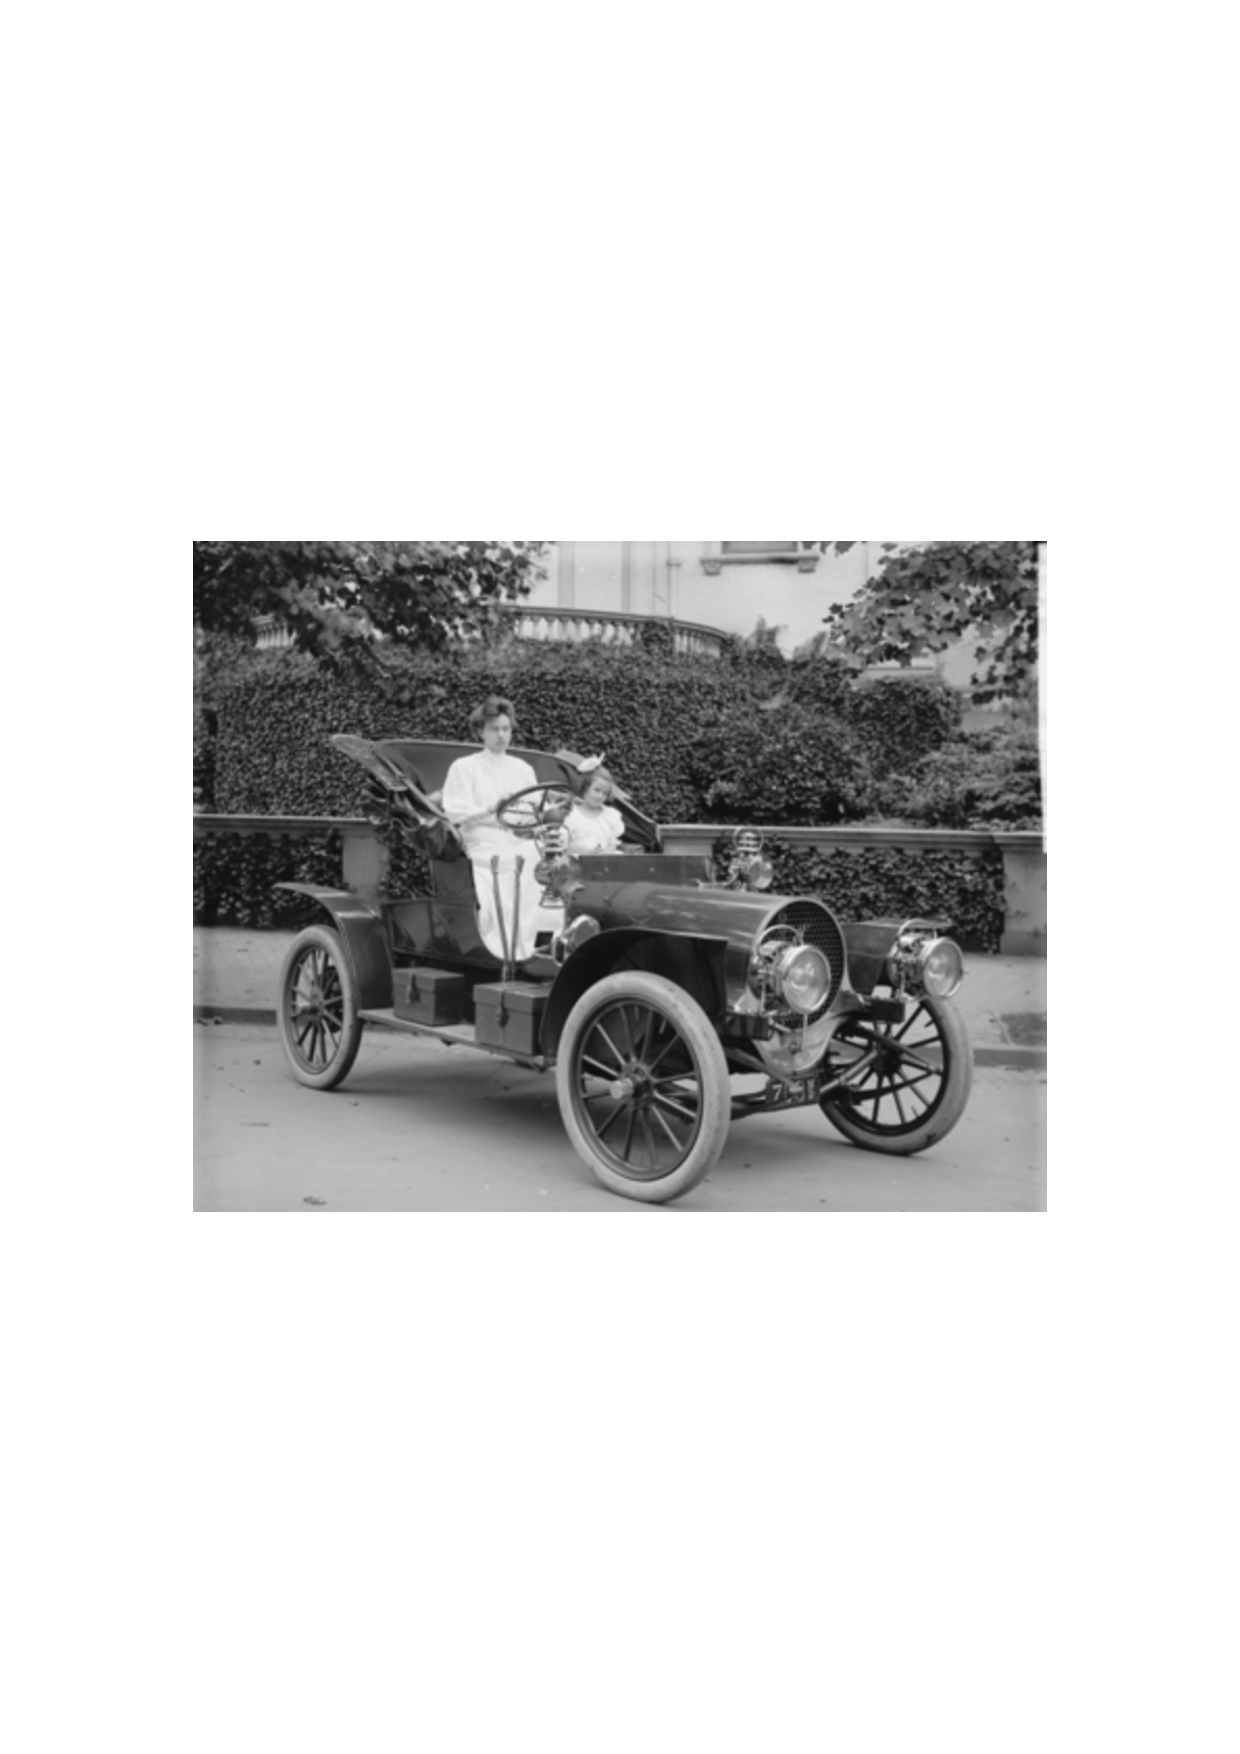
\includegraphics[width=0.8\linewidth]{figure/sample.pdf}
  \caption{1907 Franklin Model D roadster. Photograph by Harris \& Ewing, Inc. [Public domain], via Wikimedia Commons. (\url{https://goo.gl/VLCRBB}).}
  \label{fig:sample-figure}
\end{figure}

\subsection{Tables}

Put the caption above the table. Example of reference to Table~\ref{tab:sample-table}.

\begin{table}
  \caption{Frequency of Special Characters}
  \label{tab:sample-table}
  \centering
  \begin{tabular}{|c|c|l|}
    \toprule
    Non-English or Math&Frequency&Comments\\
    \midrule
    \O & 1 in 1,000& For Swedish names\\
    $\pi$ & 1 in 5& Common in math\\
    \$ & 4 in 5 & Used in business\\
    $\Psi^2_1$ & 1 in 40,000& Unexplained usage\\
  \bottomrule
\end{tabular}
\end{table}

See the \texttt{booktab} packaged documentation for further options.

\subsection{Bibliography}

Example of citations:
\begin{itemize}
	\item name: \citet{Salton1968}
	\item parenthesis: \citep{Salton1968}
\end{itemize}

An initial list of references is provided in the files \texttt{bibliography.bib} and \texttt{proceedings.bib} that you can expand.

See the \texttt{natbib} packaged documentation for further options.

\subsection{Acronyms}

Use the 

\begin{verbatim}
 \ac{acronym}
 \end{verbatim}

command to insert acronyms, eg. \ac{AP}. The command will expand the acronym the first time it is used.

An initial list of acronyms is provided in the file \texttt{acronyms.tex} that you can expand.

See the \texttt{acronym} packaged documentation for further options.


%% Define the bibliography file to be used
\bibliography{bibliography,proceedings}

\input{acronyms}


\end{document}
